

\subsection{Examples}\label{ss:ex}

Write $\nu=\tEU{p}{q}{[1,2]}$, $\mu_1=\mathrm{AG}_{[0,4]}\nu$ and
$\mu_2=\mathrm{AG}_{[0,3]}\neg q$, so $M=4$. Since
$\mathrm{AG}_\kI\chi\equiv\mathrm{A}(\bot\,\mathbf{R}_\kI\,\chi)$, the released formula
is $\varphi=\bot$ and the stop branch of \ruleref{Runf_in} always closes: a bounded
$\mathrm{AG}$ survives only through its go branch. The two runs (Fig.~\ref{fig:ex})
differ by one conjunct.

\begin{figure}[t]
\centering
\begin{subfigure}[t]{0.49\textwidth}\centering
\resizebox{\linewidth}{!}{%
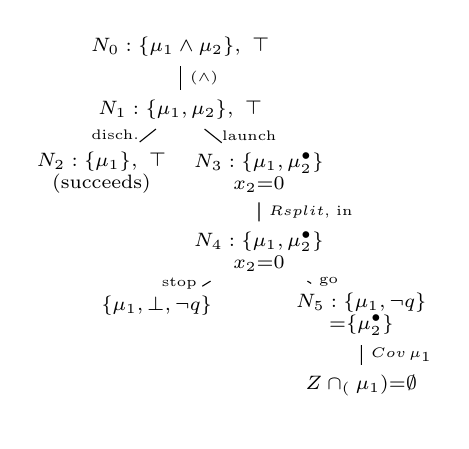
\begin{tikzpicture}[
  every node/.style={align=center, font=\scriptsize},
  level 1/.style={level distance=8mm},
  level 2/.style={sibling distance=20mm, level distance=8mm},
  level 3/.style={level distance=10mm},
  level 4/.style={sibling distance=26mm, level distance=8mm},
  level 5/.style={level distance=10mm},
  edge from parent/.style={draw,-}
]
\node {$N_0:\{\mu_1\wedge\mu_2\},\ \top$}
 child { node {$N_1:\{\mu_1,\mu_2\},\ \top$}
   child { node {$N_2:\{\mu_1\},\ \top$\\ (succeeds)}
     edge from parent node[left,font=\tiny,pos=.45]{disch.} }
   child { node {$N_3:\{\mu_1,\mu_2^\bullet\}$\\ $x_2{=}0$}
     child { node {$N_4:\{\mu_1,\mu_2^\bullet\}$\\ $x_2{=}0$}
       child { node {$\{\mu_1,\bot,\neg q\}$\\ $\CLOSED$}
         edge from parent node[left,font=\tiny,pos=.5]{stop} }
       child { node {$N_5:\{\mu_1,\neg q\}$\\ $\Ctx{=}\{\AX\mu_2^\bullet\}$}
         child { node {$Z\cap\Sat_\Ctx(\mu_1){=}\emptyset$\\ $\CLOSED$}
           edge from parent node[right,font=\tiny,pos=.5]{$\rlink{Cov}\,\mu_1$} }
         edge from parent node[right,font=\tiny,pos=.5]{go} }
       edge from parent node[right,font=\tiny]{$\rlink{Rsplit}$, in} }
     edge from parent node[right,font=\tiny,pos=.45]{launch} }
   edge from parent node[right,font=\tiny]{$(\wedge)$} };
\end{tikzpicture}}
\subcaption{$\mu_1\wedge\mu_2$: \UNSAT.}\label{fig:ex-unsat}
\end{subfigure}
\hfill
\begin{subfigure}[t]{0.49\textwidth}\centering
\resizebox{\linewidth}{!}{%
\begin{tikzpicture}[
  every node/.style={align=center, font=\scriptsize},
  level 1/.style={sibling distance=20mm, level distance=8mm},
  level 2/.style={level distance=10mm},
  level 3/.style={sibling distance=15mm, level distance=9mm},
  level 4/.style={sibling distance=20mm, level distance=9mm},
  level 5/.style={level distance=8mm},
  edge from parent/.style={draw,-}
]
\node {$N_0:\{\mu_1\},\ \top$}
 child { node (free) {$N_1:\{\,\},\ \top$\\ $\OPEN$}
   edge from parent node[left,font=\tiny,pos=.45]{disch.} }
 child { node {$N_2:\{\mu_1^\bullet\}$\\ $x_1{=}0$}
   child { node {$N_3:\{\mu_1^\bullet\}$\\ $x_1{=}0$}
     child { node {$\{\bot,\nu\}$\\ $\CLOSED$}
       edge from parent node[left,font=\tiny,pos=.5]{stop} }
     child { node {$N_4:\{\nu\}$\\ $\Ctx{=}\{\AX\mu_1^\bullet\}$}
       child { node {$N_5:\{\nu^\bullet\}$\\ $x_\nu{=}0$}
         child { node {$\{p,\EX\nu^\bullet\}$}
           child { node {$\{q\},\ x_\nu\in[1,2]$\\ $\OPEN$}
             edge from parent node[right,font=\tiny,pos=.5]{$\rlink{Delay}$, $\rlink{EX}$} }
           edge from parent node[right,font=\tiny,pos=.5]{$\rlink{Ugo}$} }
         edge from parent node[right,font=\tiny,pos=.5]{$\rlink{Cov}\,\nu$} }
       edge from parent node[right,font=\tiny,pos=.5]{go} }
     edge from parent node[right,font=\tiny]{$\rlink{Rsplit}$, in} }
   edge from parent node[right,font=\tiny,pos=.45]{launch} };
\draw[->,dashed] (free.west) to[out=200,in=160,looseness=3.4]
  node[left=3pt,font=\tiny]{stutter} ([yshift=-3pt]free.north west);
\end{tikzpicture}}
\subcaption{$\mu_1$ alone: \SAT.}\label{fig:ex-sat}
\end{subfigure}
\caption{Tableau runs, with $\nu=\tEU{p}{q}{[1,2]}$, $\mu_1=\mathrm{AG}_{[0,4]}\nu$,
$\mu_2=\mathrm{AG}_{[0,3]}\neg q$.}\label{fig:ex}
\end{figure}

\begin{example}[$\mu_1\wedge\mu_2$]\label{ex:unsat}
After $(\wedge)$, covering $\mu_2$ succeeds under the empty context and splits $N_1$
into a discharge child and a launch child $N_3$, which carries $\mu_1$ alongside the
pursuit. At $N_3$ the zone is the point $x_2{=}0$, so \ruleref{Rsplit} leaves only its
in-part; \ruleref{Runf_in} closes the stop child on $\bot$ and yields $N_5$, where the
context now forces $\neg q$ wherever $x_2\in[0,3]$.

Covering $\mu_1$ there fails. Computing $\Sat_\Ctx(\mu_1)$ unfolds it to a demand for
$\nu$ at the onset, and unfolding $\nu$ by \ruleref{Uunf} closes both branches:
\ruleref{Ustop} lands on $x_\nu\in[1,2]$, which coincides with $x_2\in[1,2]\subseteq[0,3]$,
so the node carries $q$ and $\neg q$; \ruleref{Ugo} defers with no deadline to cap it, and
once $x_\nu>2$ the window has passed with the stop never taken, so every repeat fails
acceptance condition~(i). Hence $\Sat_\Ctx(\nu)=\emptyset$ at this onset,
$Z\cap\Sat_\Ctx(\mu_1)=\emptyset$, and neither \ruleref{Cov} nor \ruleref{Covstar} applies:
$N_5$ closes and the formula is \UNSAT. The calculus never compares the two modalities
directly; it only brings $q$ and $\neg q$ into one goal set over overlapping zones.
\end{example}

\begin{example}[$\mu_1$ alone]\label{ex:sat}
Without $\mu_2$ nothing constrains $q$, so covering $\nu$ at $N_4$ succeeds and launches
its pursuit with $x_\nu$ reset. That pursuit shows how a window is entered: at $N_5$ the
zone is $x_\nu{=}0$, so \ruleref{Ustop} has empty zone and closes, and only \ruleref{Ugo}
survives, asserting $p$ and deferring $\EX\nu^\bullet$. The resulting node is saturated,
so \ruleref{Delay} advances the zone and \ruleref{EX} supplies the successor carrying
$\nu^\bullet$; at the first one with $x_\nu\in[1,2]$ the stop child is consistent and the
eventuality is fulfilled.

Meanwhile $\AX\mu_1^\bullet$ rides every successor, re-imposing $\mu_1$ across its window.
Once $x_1>4$ the after-part of \ruleref{Rsplit} drops $\mu_1^\bullet$, leaving a goal-free
node whose stutter loop is accepting: no until pursuit is active, so condition~(i) is
vacuous, and $x_1$ is extrapolated above $M{=}4$. The cycle can only live in this lapsed
tail, since inside the window the release's own split bounds $x_1$. The marking succeeds,
and reading it off gives a one-location automaton labelled $p$ with a $q$-successor
reachable within $[1,2]$ of each onset.
\end{example}